\documentclass{standalone}
\usepackage{pgf,tikz}
\usepackage{bm}

\begin{document}

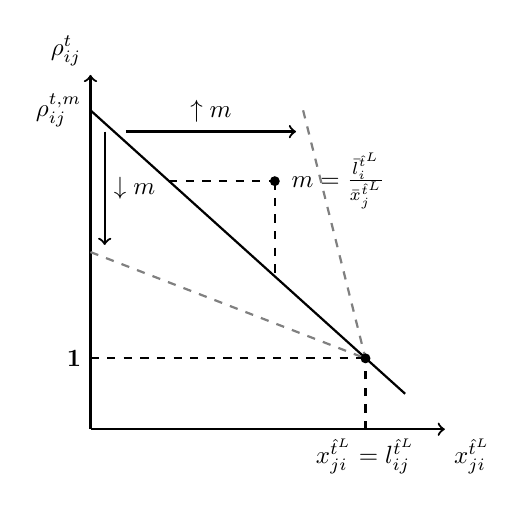
\begin{tikzpicture}[thick,scale=0.9, every node/.style={scale=0.9}]


% Graph axes
\draw[thick,->] (0,0) -- (5,0) node[anchor=north west] {$x_{ji}^{\hat{t}^{L}}$};
\draw[thick,->] (0,0) -- (0,5)  node[anchor=south east] {$\rho_{ij}^{t}$};

% Linear functions
\draw (0,4.5) coordinate (c_1) node[left] {$\rho_{ij}^{t,m}$}  -- (4.44,0.5) coordinate (c_2);

\draw [dashed, gray] (3,4.5) to (3.88,1);
    \draw [->] (0.5,4.2) to node [midway, above] {$\uparrow m$} (2.9,4.2);
\draw [dashed, gray] (0,2.5) to (3.88,1);
    \draw[->] (0.2,4.2) to node [midway, right] {$\downarrow m$} (0.2,2.6);

% Various labels
\node [below] at(3.88,0) {$x_{ji}^{\hat{t}^{L}}=l_{ij}^{\hat{t}^{L}}$};

\node at (3.5,3.5) {$m=\frac{\bar{l}_{i}^{\hat{t}^{L}}}{\bar{x}_{j}^{\hat{t}^{L}}}$};

% Horizontal dashed lines
\draw[dashed] (0,1) coordinate (h1_1) node[left] {$\bm{1}$} -- (3.88,1) coordinate (h1_2);
\draw[dashed] (1.11,3.5) coordinate (h2_1) -- (2.6,3.5) coordinate (h2_2);


% Vertical dashed lines

\draw[dashed] (3.88,0) coordinate (v1_1) -- (3.88,1) coordinate (v1_2);
\draw[dashed] (2.6,3.5) coordinate (v2_1) -- (2.6,2.16) coordinate (v2_2);

% Various intersections

%\coordinate (i6) at (intersection of c_1--c_2 and d_1--d_2);
%\fill[black] (i6) circle (2pt);

\coordinate (i7) at (intersection of h1_1--h1_2 and v1_1--v1_2);
\fill[black] (i7) circle (2pt);

\coordinate (i8) at (intersection of h2_1--h2_2 and v2_1--v2_2);
\fill[black] (i8) circle (2pt);

%\coordinate (i8) at (intersection of h3_1--h3_2 and v3_3--v3_4);
%\fill[black] (i8) circle (2pt);
%
%\coordinate (i9) at (intersection of h4_1--h4_2 and v4_1--v4_2);
%\fill[black] (i9) circle (2pt);

%\coordinate (i10) at (intersection of h4_1--h4_2 and v4_3--v4_4);
%\fill[black] (i10) circle (2pt);

% Labels

%\node[draw=none] at (2.5,-1) {\textit{(a)}};
%\node[draw=none] at (12.5,-1) {\textit{(b)}};



\end{tikzpicture}

\end{document}